\section{Test Description and Success Criteria}
This test is located in \texttt{simulation/dynamics/sphericalPendulum/UnitTest/\newline
test\_sphericalPendulum.py}. In this integrated test there are two spherical pendulums connected to the spacecraft hub.  There are two scenarios being tested: one with the time step being 0.01 and one with the time step 0.001. Both tests should show energy and momentum conservation but the 0.001 should show less integration error. 

\section{Test Parameters}

To validate and test the code a simulation with two spherical pendulums has been run using the following input parameters:
\begin{align}
\begin{split}
l_1=0.3 m, \qquad m_1=20 kg, \qquad \dot{\varphi}_{1,0}=0.01 rad/s, \qquad \dot{\vartheta}_{1,0}= 0.05 rad/s \\
\bm{d}_1=
\begin{bmatrix}
0.1 \\
0.1 \\
0.1\\
\end{bmatrix} m
\qquad
\qquad
\bm{\hat{p}}_{0_1,1}=
\begin{bmatrix}
\sqrt{2}/2 \\
0 \\
\sqrt{2}/2\\
\end{bmatrix}
\qquad
\bm{\hat{p}}_{0_1,2}=
\begin{bmatrix}
0 \\
1 \\
0\\
\end{bmatrix}
\qquad
\bm{\hat{p}}_{0_1,3}=
\begin{bmatrix}
-\sqrt{2}/2 \\
0 \\
\sqrt{2}/2\\
\end{bmatrix}
\end{split}
\end{align}

\begin{align}
\begin{split}
l_2=0.4 m, \qquad m_2=40 kg, \qquad \dot{\varphi}_{2,0}=0.1 rad/s, \qquad \dot{\vartheta}_{2,0}= 0.5 rad/s \\
\bm{d}_1=
\begin{bmatrix}
0.1 \\
0.1 \\
0.1\\
\end{bmatrix} m
\qquad
\bm{\hat{p}}_{0_2,1}=
\begin{bmatrix}
1 \\
0 \\
0\\
\end{bmatrix}
\qquad
\bm{\hat{p}}_{0_2,2}=
\begin{bmatrix}
0 \\
1 \\
0\\
\end{bmatrix}
\qquad
\bm{\hat{p}}_{0_2,3}=
\begin{bmatrix}
0 \\
0 \\
1 \\
\end{bmatrix}
\end{split}
\end{align}

\begin{table}[htbp]
	\caption{Error Tolerance - Note: Relative Tolerance is $\textnormal{abs}(\frac{\textnormal{truth} - \textnormal{value}}{\textnormal{truth}}$)}
	\label{tab:errortol}
	\centering \fontsize{10}{10}\selectfont
	\begin{tabular}{| c | c |} % Column formatting, 
		\hline
		Test   & Relative Tolerance \\
		\hline
		Energy and Momentum Conservation & 1e-8 \\
		\hline	
	\end{tabular}
\end{table}

\section{Test Results}

The following figures show the conservation of the quantities described in the success criteria for each scenario. The conservation plots are all relative difference plots. All conservation plots show integration error which is the desired result. In the python test these values are automatically checked therefore when the tests pass, these values have all been confirmed to be conserved. An additional note: the angular momentum plots are plotting the change in the components of the angular momentum vector in the inertial frame. The individual components are not labeled because the goal is for each component to show conservation therefore the individual components do not have separate information needing to be specified.  

\subsection{Time Step = 0.01}
\begin{figure}[htbp]
	\centerline{
		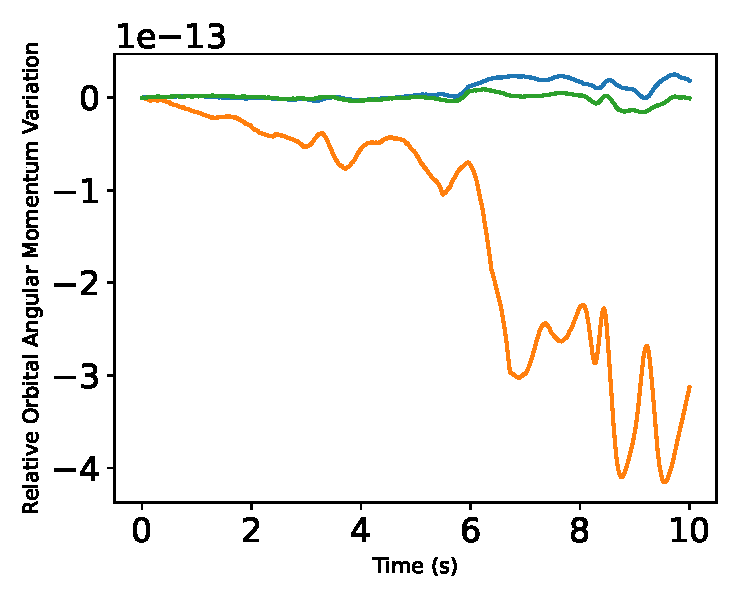
\includegraphics[width=0.8\textwidth]{AutoTeX/ChangeInOrbitalAngularMomentumOneHundredth.pdf}}
	\caption{Change in Orbital Angular Momentum Time Step = 0.01}
	\label{fig:ChangeInOrbitalAngularMomentumTimeStep01}
\end{figure}
\begin{figure}[htbp]
	\centerline{
		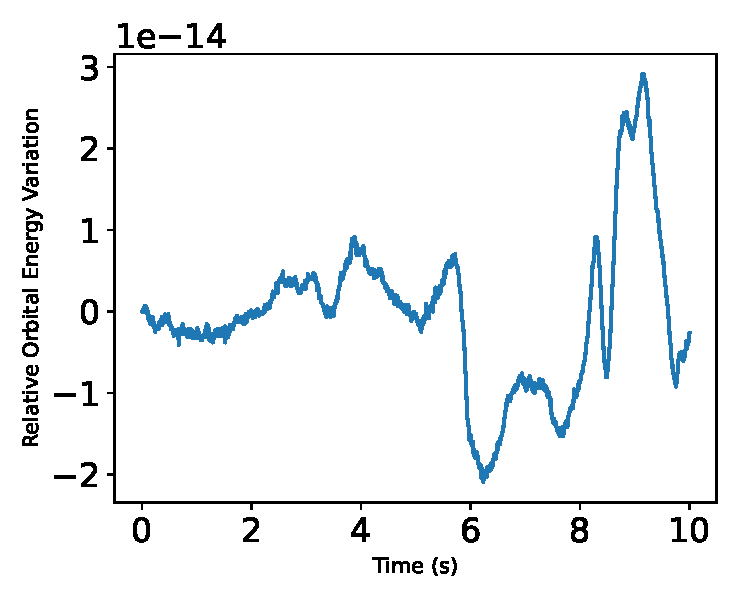
\includegraphics[width=0.8\textwidth]{AutoTeX/ChangeInOrbitalEnergyOneHundredth.pdf}}
	\caption{Change in Orbital Energy Time Step = 0.01}
	\label{fig:ChangeInOrbitalEnergyTimeStep01}
\end{figure}
\begin{figure}[htbp]
	\centerline{
		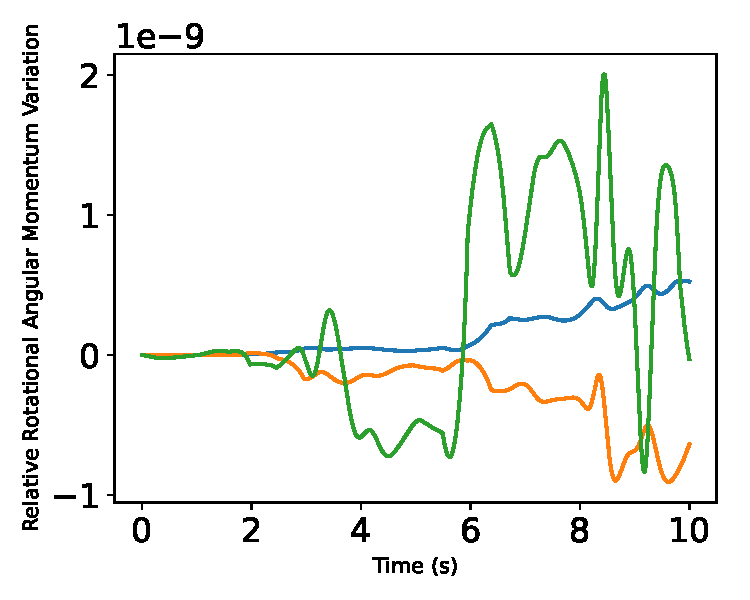
\includegraphics[width=0.8\textwidth]{AutoTeX/ChangeInRotationalAngularMomentumOneHundredth.pdf}}
	\caption{Change In Rotational Angular Momentum Time Step = 0.01}
	\label{fig:ChangeInRotationalAngularMomentumTimeStep01}
\end{figure}
\begin{figure}[htbp]
	\centerline{
		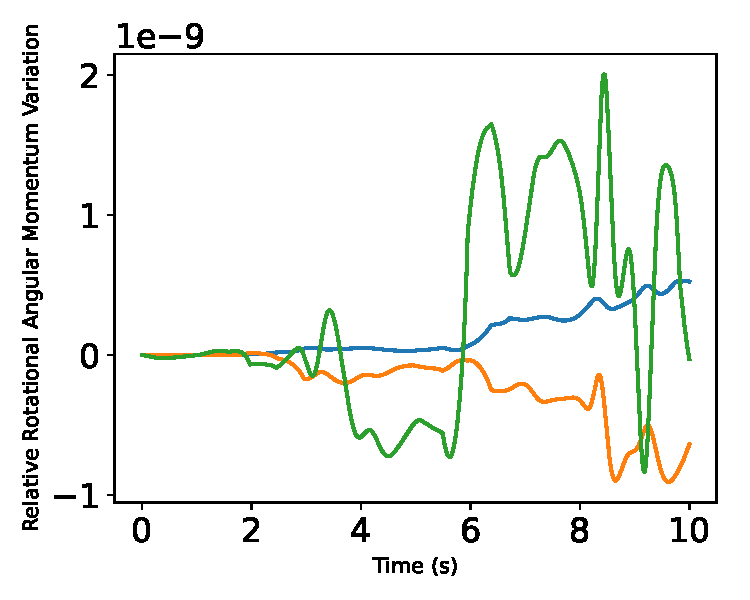
\includegraphics[width=0.8\textwidth]{AutoTeX/ChangeInRotationalAngularMomentumOneHundredth.pdf}}
	\caption{Change In Rotational Energy Time Step = 0.01}
	\label{fig:ChangeInRotationalEnergyTimeStep01}
\end{figure}
\clearpage

\subsection{Time Step = 0.001}
\begin{figure}[htbp]
	\centerline{
		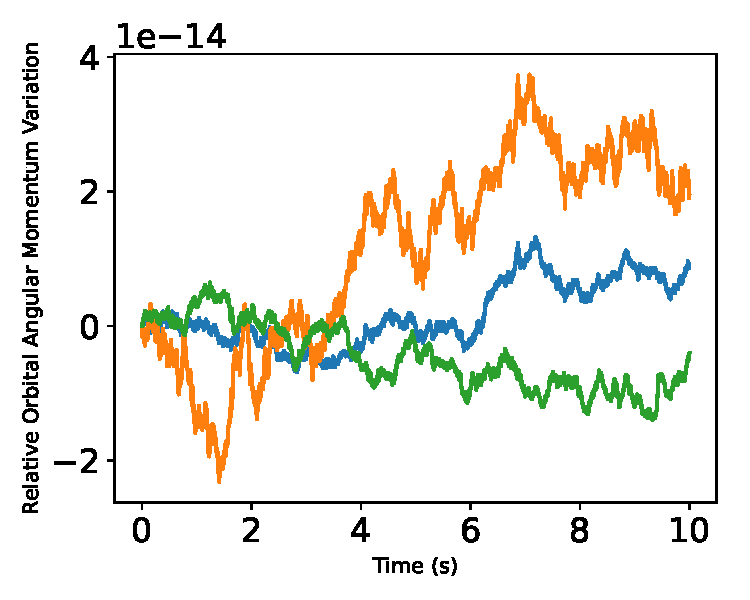
\includegraphics[width=0.8\textwidth]{AutoTeX/ChangeInOrbitalAngularMomentumOneThousandth.pdf}}
	\caption{Change in Orbital Angular Momentum Time Step = 0.001}
	\label{fig:ChangeInOrbitalAngularMomentumTimeStep001}
\end{figure}
\begin{figure}[htbp]
	\centerline{
		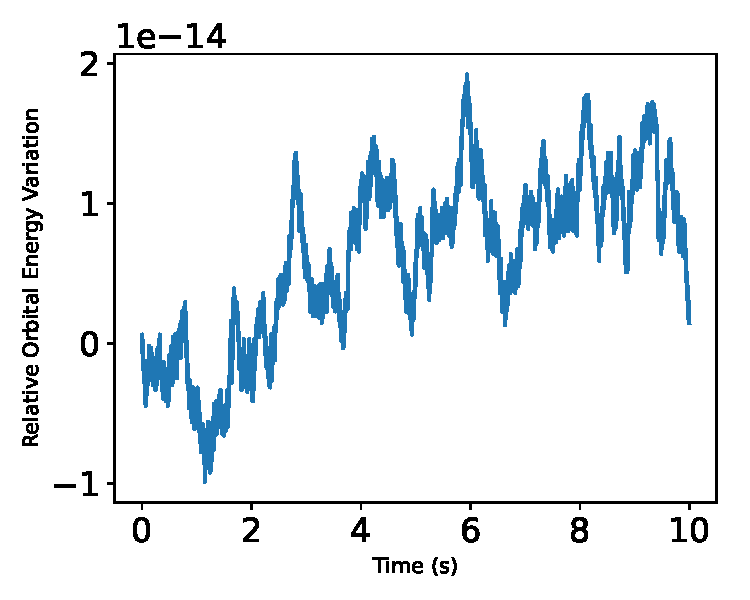
\includegraphics[width=0.8\textwidth]{AutoTeX/ChangeInOrbitalEnergyOneThousandth.pdf}}
	\caption{Change in Orbital Energy Time Step = 0.001}
	\label{fig:ChangeInOrbitalEnergyTimeStep001}
\end{figure}
\begin{figure}[htbp]
	\centerline{
		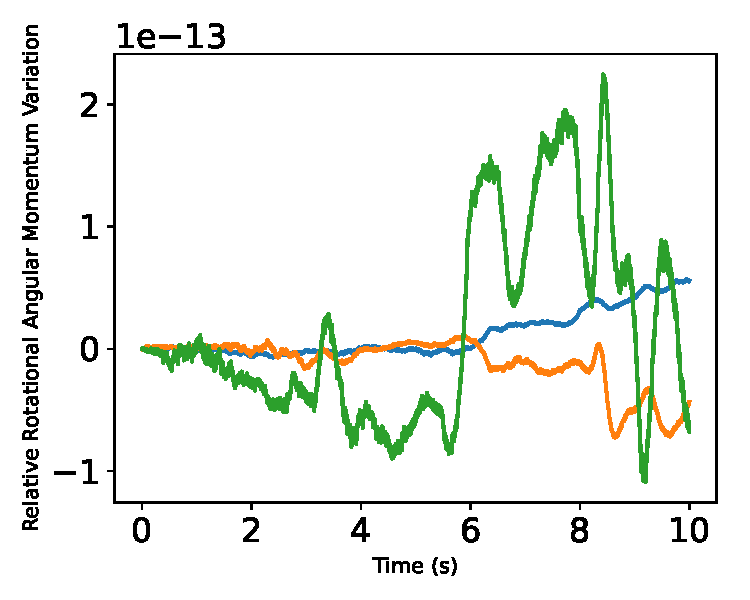
\includegraphics[width=0.8\textwidth]{AutoTeX/ChangeInRotationalAngularMomentumOneThousandth.pdf}}
	\caption{Change In Rotational Angular Momentum Time Step = 0.001}
	\label{fig:ChangeInRotationalAngularMomentumTimeStep001}
\end{figure}
\begin{figure}[htbp]
	\centerline{
		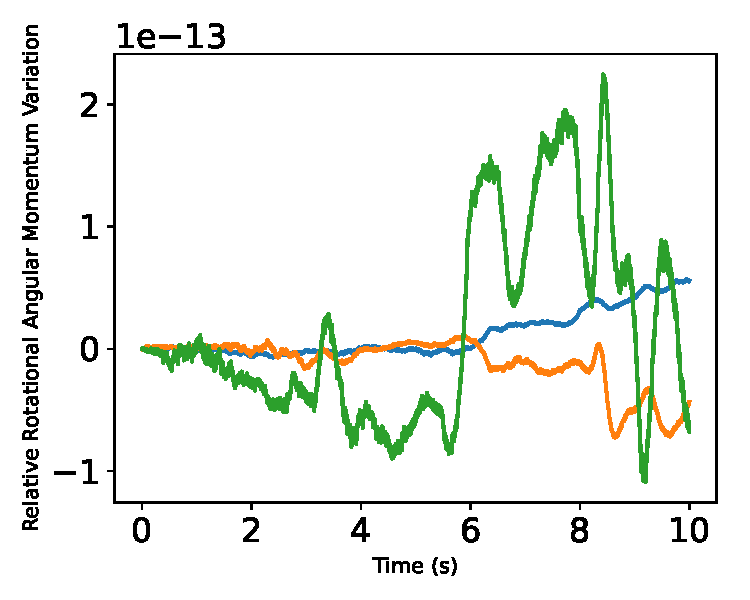
\includegraphics[width=0.8\textwidth]{AutoTeX/ChangeInRotationalAngularMomentumOneThousandth.pdf}}
	\caption{Change In Rotational Energy Time Step = 0.001}
	\label{fig:ChangeInRotationalEnergyTimeStep001}
\end{figure}
\clearpage
